\section{<<Crossing the river>>}

\begin{figure}[h]
  \label{fig:cross}
  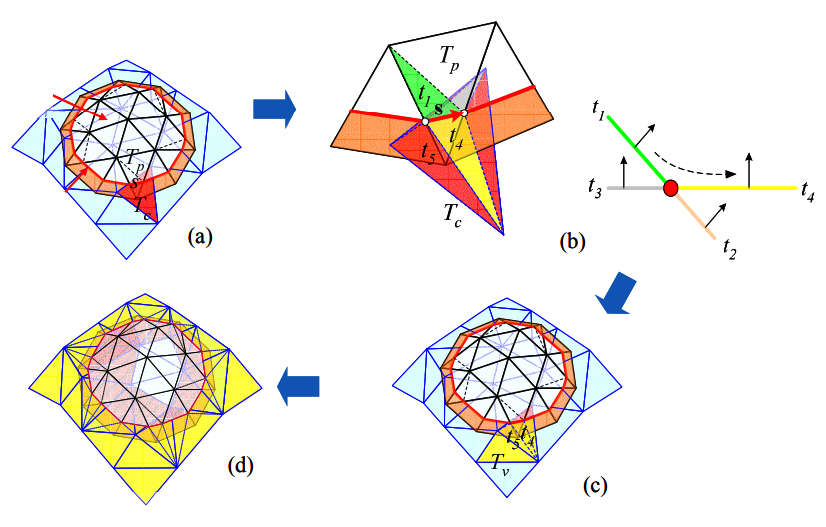
\includegraphics[width=0.7\linewidth]{36.png}
  \centering
  \caption{подробные шаги <<crossing the river>>}
\end{figure}

Процесс построения \textit{валидного региона} может распространиться за самопересечение и переместиться к подтреугольникам соседнего треугольника. Рисунок $2.1$ иллюстрирует подробные шаги распространия внутри подтреугольников частично валидного треугольника. Все начинается с триангуляции соседнего треугольника $T_c$ как в секции 2.5. На рисунке (b) есть два треугольника $t_3$, $t_4$, смежных с ребром-входом. Подтреугольник $t_4$ выбирается как валидный, и будет служить как начальный треугольник в процессе построения внутри подтреугольников $T_c$. В конце концов, как показано на рисунке (c), треугольник $T_v$ будет найден как валидный треугольник и будет добавлен в $\mathbf{S}$.


